%Modify the relative path accordingly
%HU, Pili
%Create: 20120330
%Modify: 20120330
%The unified entry to include in my tutorial series

%HU, Pili
%Create: 20110910
%Modify: 20120330
%purpose of this file is to gather commonly used
%mathematical abbreviations, to speed up writing
%notes

\documentclass[11pt,a4paper]{article}
\usepackage[utf8x]{inputenc}
\usepackage{ucs}
\usepackage{amsmath}
\usepackage{amsfonts}
\usepackage{amssymb}
\usepackage{amsthm}
\usepackage{url}
\usepackage{graphicx}

\usepackage{fancyhdr}
\pagestyle{fancy}
\fancyhead{}

%=====Calculus======
%the following commands are not originated by me
%I pick them from http://www-solar.mcs.st-and.ac.uk/~clare/Latex/
%the following line controls the style of patial derivative
%1), use \dfrac, height is larger, looks good. 
%2), use \frac, also work, but space looks limited. 
\newcommand{\myfrac}[2]{\dfrac{#1}{#2}}
\newcommand{\diff}[2]{\myfrac{{\rm d}#1}{{\rm d}#2}}
\newcommand{\ndiff}[3]{\myfrac{{\rm d}^{#3}#1}{{\rm d}#2^{#3}}}
\newcommand{\pdiff}[2]{\myfrac{\partial #1}{\partial #2}}
\newcommand{\npdiff}[3]{\myfrac{\partial^{#3} #1}{\partial #2^{#3}}}
\newcommand{\e}[1]{\ensuremath{{\rm e}^{#1}}}
\newcommand{\ldiff}[2]{\ensuremath{{\rm d}#1/{\rm d}#2}}
\newcommand{\lpdiff}[2]{\ensuremath{\partial#1/\partial#2}}
\newcommand{\lnpdiff}[3]{\ensuremath{\partial^{#3}#1/\partial#2^{#3}}}
\newcommand{\dif}[1]{\mathrm{d}#1}

%20120330
%The reason I don't copy the original file as a whole
%is that it contains too many individually preferred 
%definitions. 
%
%I start with those basic symbols and adapt them in use. 

%=====Matrix======
\newcommand{\tr}[1]{\mathrm{Tr}\left[#1\right]}
\newcommand{\tran}[1]{#1^\mathrm{T}}
%The following shorthand of matrix may be convenient. 
%However, it is so short that I'm worried it may 
%collide with something else. I don't use at present.
%\newcommand{\m}[1]{\mathbf{#1}}
\newcommand{\adj}[0]{\mathrm{adj}}

%=====Theorem definitions=====
\newcounter{mytheoremorder}
\newtheorem{mydef}{Definition}
\newtheorem{myaxm}{Axiom}
\newtheorem{mythm}[mytheoremorder]{Theorem}
\newtheorem{myprop}[mytheoremorder]{Proposition}
\newtheorem{myex}{Example}

%=====Optimization====
\DeclareMathOperator*{\argmax}{arg\,max}
\DeclareMathOperator*{\argmin}{arg\,min}
\newcommand{\maximize}[0]{\mathrm{Maximize~}}
\newcommand{\minimize}[0]{\mathrm{Minimize~}}

%=====Probability====
\newcommand{\E}[0]{\mathbb{E}}
\newcommand{\var}[0]{\mathrm{Var}}
\newcommand{\cov}[0]{\mathrm{Cov}}

%=====Quick and Unified Reference====
%20120505
%Usage: \eq{\ref{xxx}}
%The reason I keep "\ref" away from definition, 
%and let user type it every time is that: 
%currently I'm working on Texmaker, and it can 
%trigger a selection panel when the sequence 
%"\ref" is found. Maybe further configuration of 
%texmake can make it do the same thing when the 
%following self-defined sequence is detected.
%This is left for future work. 
\newcommand{\req}[1]{\textbf{Eq~{#1}}}
\newcommand{\rfig}[1]{\textbf{Fig~{#1}}}
\newcommand{\rtbl}[1]{\textbf{Tbl~{#1}}}
\newcommand{\rpg}[1]{\textbf{P~{#1}}}
\newcommand{\rsec}[1]{\textbf{Section~{#1}}}


\usepackage{algorithm}
\usepackage{algorithmic}
\floatname{algorithm}{Algorithm}
\renewcommand{\algorithmicrequire}{\textbf{Input:}}
\renewcommand{\algorithmicensure}{\textbf{Output:}}

%notation shortcuts
\newcommand{\nL}{\mathcal{L}}
\newcommand{\nA}{\mathcal{A}}
\newcommand{\sym}[1]{#1_{\text{sym}}}
\newcommand{\rw}[1]{#1_{\text{rw}}}
\newcommand{\cut}[1]{\text{cut}(#1)}
\newcommand{\assoc}[1]{\text{assoc}(#1)}
\newcommand{\vol}[1]{\text{vol}(#1)}
%Moore-Penrose Inverse
%I can not find that "plus" look symbol
%Currently use "plus"..
\newcommand{\mpinv}{+}


\usepackage{subfigure}

\fancyhead[LO,LE]{HU, Pili}
\fancyhead[RO,RE]{Spectral Clustering Survey}

%This usually doesn't need modification 
\author{HU, Pili\thanks{hupili [at] ie [dot] cuhk [dot] edu [dot] hk}}

%Modify them accordingly===
\title{Spectral Clustering Survey}
\date{May 14, 2012\thanks{Last compile:\today}}

\begin{document}

\maketitle
%>============================================
\begin{abstract}
	Abstract. Sources can be found in \cite{hu2012-spectral2hop}. 
\end{abstract}
%<=======Abstract ENd=========================

%>============================================
\pagebreak
\setcounter{tocdepth}{3}
\tableofcontents
\pagebreak
%<=======TOC ENd==============================



\section{Introduction}
\label{sec:introduction}

Spectral Clustering(SC) was used in several disciplines long ago. 
For example, computer vision\cite{shi2000normalized}.
Spectral Embeding(SE) was 
also widely discussed in the community\cite{brand2003unifying}. 
Outside spectral community, the machine learning community also 
developed many linear or non-linear Dimensionality Reduction(DR) methods, 
like Principal Component Anslysis (PCA), Kernel PCA (KPCA)\cite{scholkopf1998kpca}, 
Locally Linear Embedding (LLE)\cite{roweis2000lle}, etc. 
Other technique like Multi-Dimensional Scaling(MDS) was successfully 
used in computational psychology for a very long time\cite{borg2005modern}, 
which can be viewed as both "embedding" or "dimensionality reduction".

%, load balancing
%\cite{hendrickson1993multidimensional}, electronics design
%\cite{hadley1992efficient}, etc.

According to our survey, although those methods target at different problems
and are derived from different assumptions, they do share a lot in common. 
The most significant sign is that, the core procedure involves 
Eigen Value Decomposition(EVD) or Singular Value Decomposition(SVD), aka "spectral". 
They all involve an intermidiate step of embedding high-dimensional / 
non-Euclidean / non-metric points into a low-dimensional Euclidean space
(although some do not embed explicitly). In this case, we categorize all 
these algorithms as Spectral Embedding Technique(SET). 


\subsection{A Sample Spectral Clustering Algorithm}

%%Following is just an example copied from:
%%http://en.wikibooks.org/wiki/LaTeX/Algorithms_and_Pseudocode
%\begin{algorithm}                      % enter the algorithm environment
%\caption{Calculate $y = x^n$}          % give the algorithm a caption
%\label{alg1}                           % and a label for \ref{} commands later in the document
%\begin{algorithmic}                    % enter the algorithmic environment
%    \REQUIRE $n \geq 0 \vee x \neq 0$
%    \ENSURE $y = x^n$
%\end{algorithmic}
%\end{algorithm}

There are many variations of SC. They all work under certain conditions
and researchers don't have a rule of thumb so far. Before we analyze their
procedure and justification, we present a simple but workable sample 
algorithm(\ralg{\ref{alg:sc_sample}}). 

\begin{algorithm}[htb]
	\caption{Sample Spectral Clustering}
	\label{alg:sc_sample}
	\begin{algorithmic}[1]
		\REQUIRE Data matrix $X = [x_1, x_2, \ldots, x_N]$;  
		Number of Clusters $K$. 
		\ENSURE Clustering $\{C_i\}$: $C_i \in V$ 
			and $\cap_i C_i = \emptyset$
			and $\cup_i C_i = V$. 
		\STATE Form adjacency matrix $A$ within $\epsilon$-ball.
		\STATE Solve $A = U \Lambda \tran{U}$, indexed according 
		the eigenvalue's magnitude. 
		\STATE $Y \leftarrow$ first $K$ columns of U. 
		\STATE Cluster $Y$'s rows by K-means. 
	\end{algorithmic}
\end{algorithm}

In \ralg{\ref{alg:sc_sample}}, the $\epsilon$-ball adjacency graph is 
constructed as follows. First create one vertex for each data point. 
If for two points $i,j$ satisfy $||x_i-x_j|| < \epsilon$, connect 
them with an edge. In this simple demonstration, we consider an unweighted
graph, i.e. all entries of $A$ are 0(disconnected) or 1(connected). 

\begin{figure}
	\centering
	\subfigure[Data Scatter Plot]{
		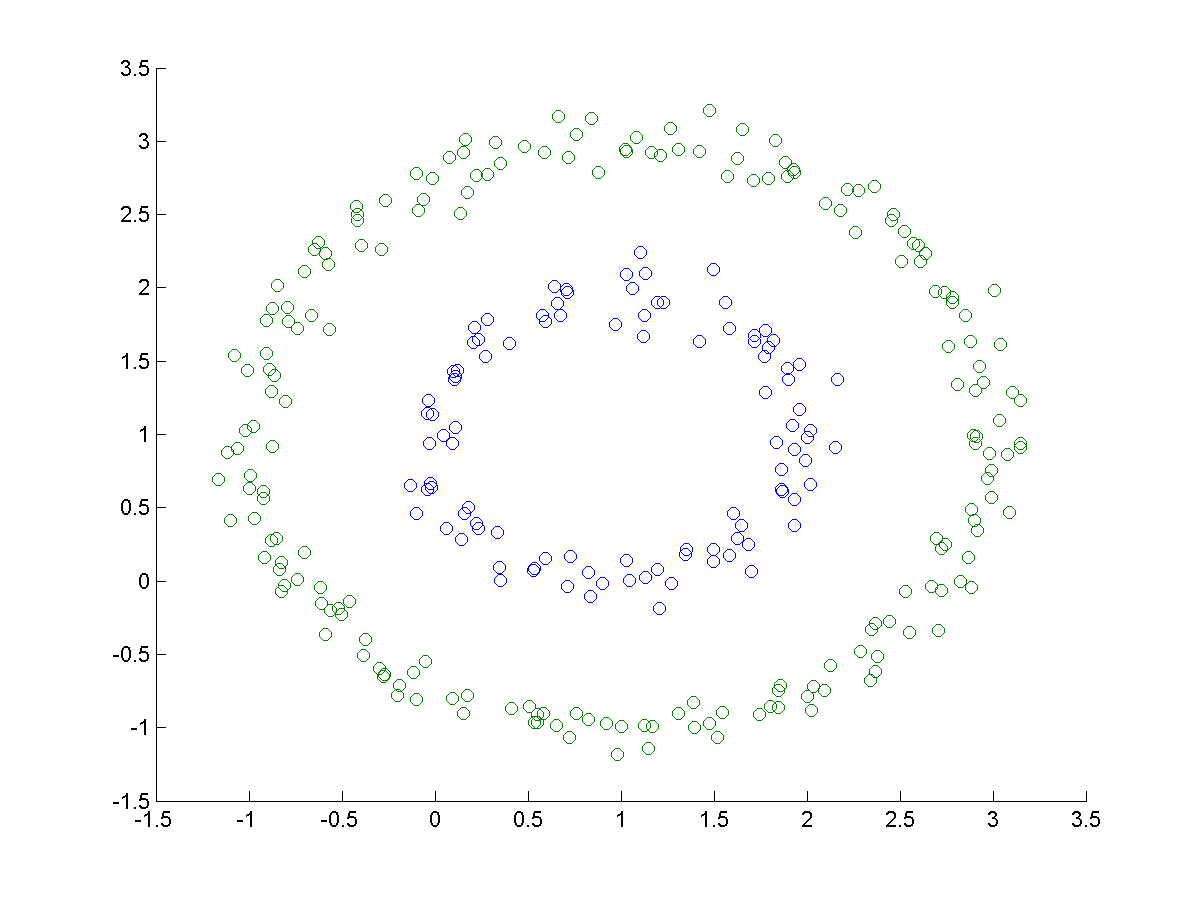
\includegraphics[width=0.4\textwidth]{../plot/sc_sample_scatter.png}	
		\label{fig:ssc_data}
	}
	\subfigure[Standard K-means]{
		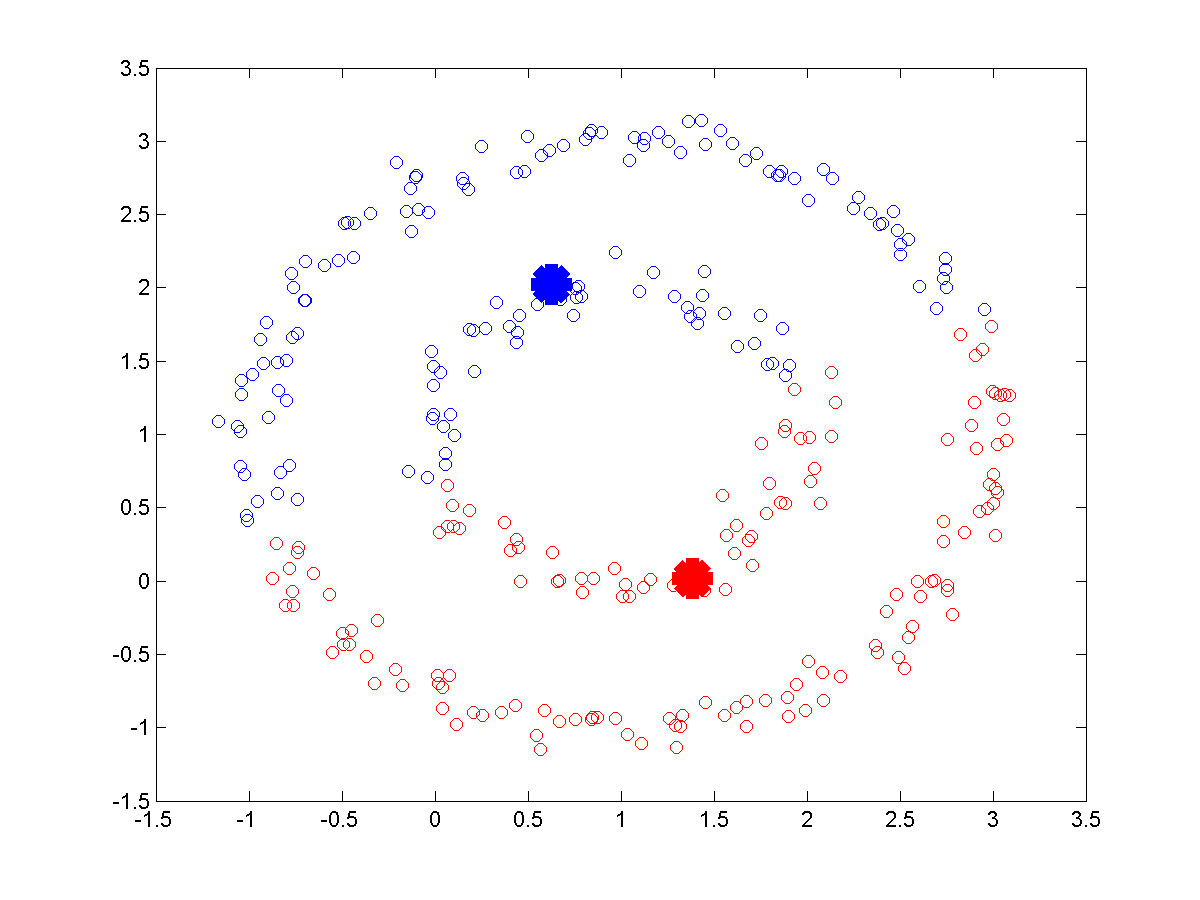
\includegraphics[width=0.4\textwidth]{../plot/sc_sample_kmeans.png}	
		\label{fig:ssc_kmeans}
	}
	\subfigure[Adjacency Graph]{
		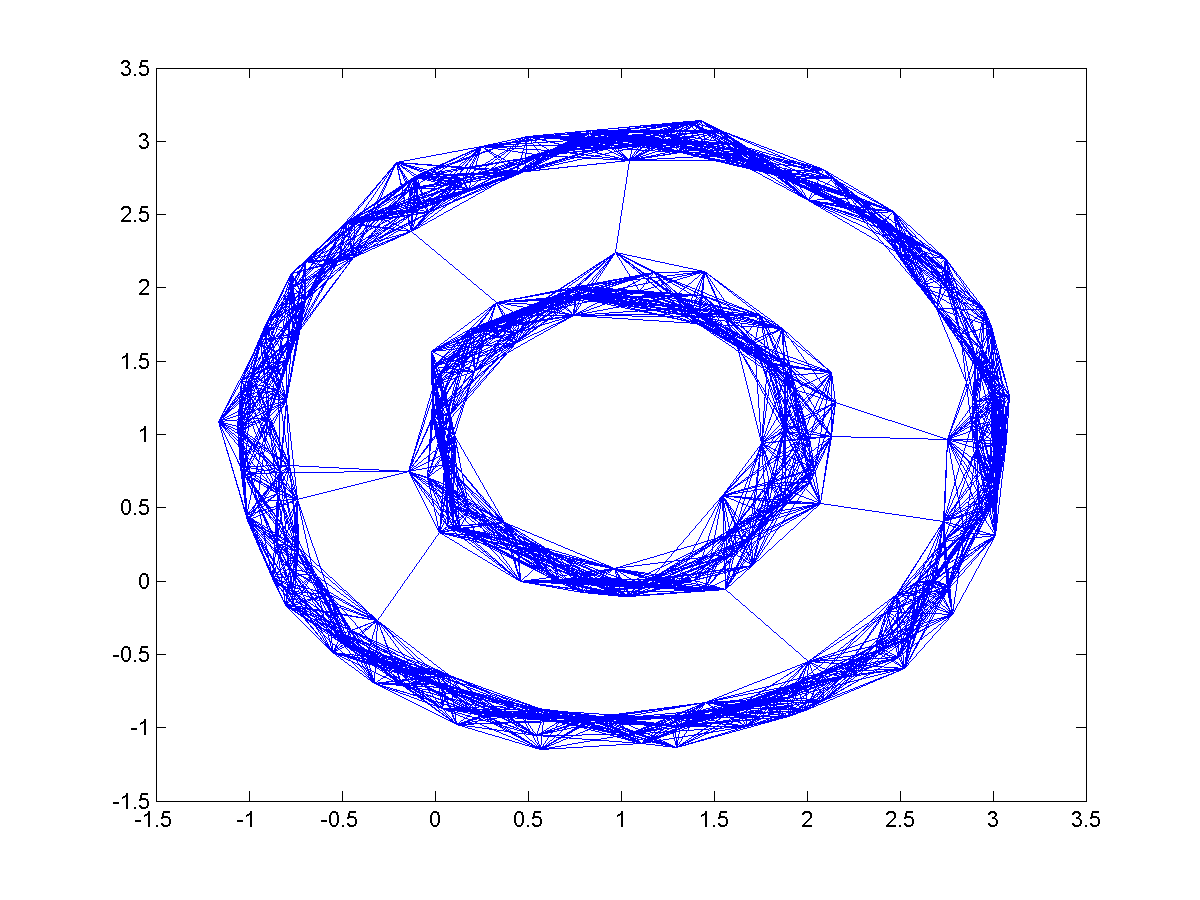
\includegraphics[width=0.4\textwidth]{../plot/sc_sample_adj.png}	
		\label{fig:ssc_adj}
	}
	\subfigure[Sample SC Algorithm]{
		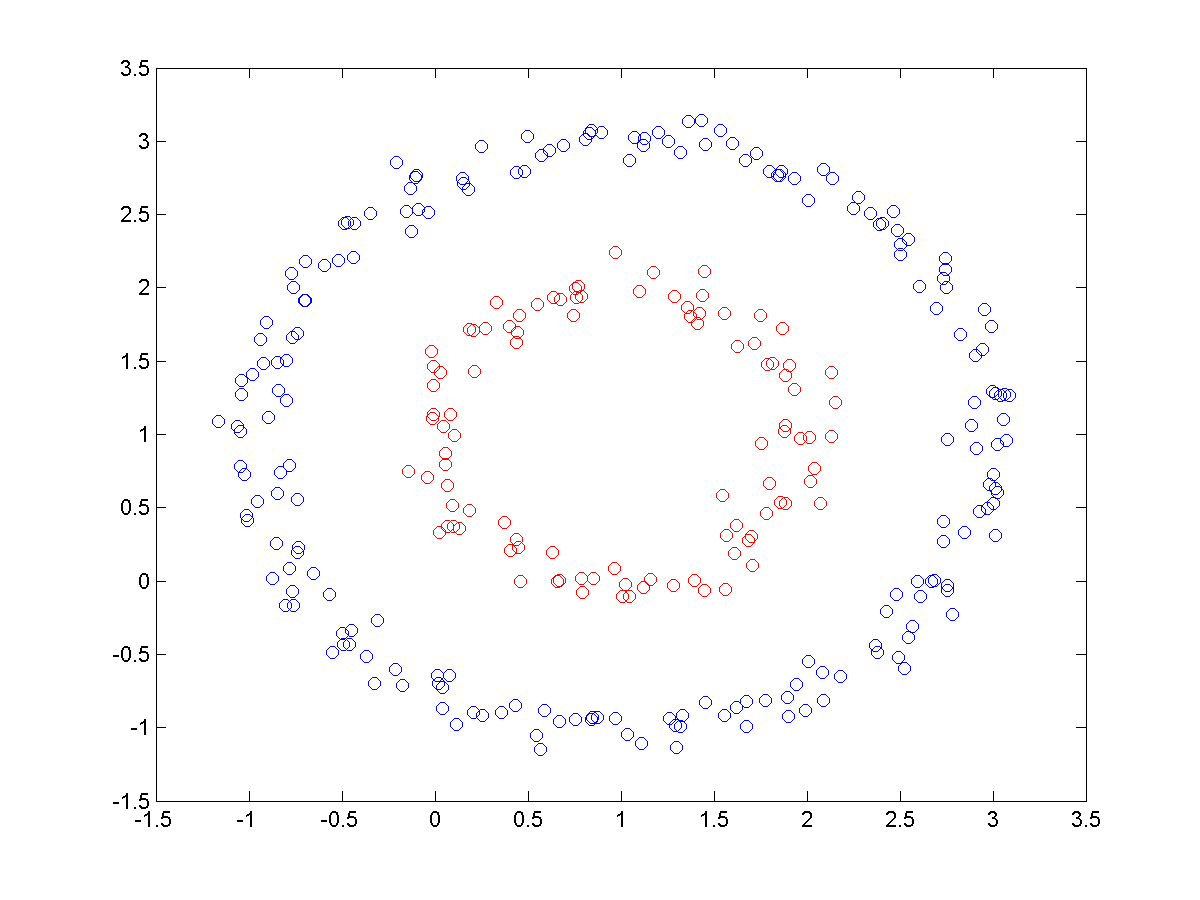
\includegraphics[width=0.4\textwidth]{../plot/sc_sample_sc.png}	
		\label{fig:ssc_sc}
	}
	\caption{Demonstration of Sample SC Algorithm}
	\label{fig:ssc_demo}
\end{figure}

\rfig{\ref{fig:ssc_demo}} demonstrates the result of our sample SC algorithm, 
compared with standard K-means algorithm. 
\rfig{\ref{fig:ssc_data}} shows the scatter plot of data. 
It is composed of one radius 1 circle and another radius 2 circle, 
both centered at (1,1). 
\rfig{\ref{fig:ssc_kmeans}} shows the result of standard K-means
working on Euclidean distance. 
\rfig{\ref{fig:ssc_adj}} shows the graph representation, where 
the adjacency graph is formed by taking a $\epsilon$-ball and 
$\epsilon=0.7$ in the example. 
\rfig{\ref{fig:ssc_sc}} shows the output of \ralg{\ref{alg:sc_sample}}. 
It's obvious that standard K-means algorithm can not correctly cluster 
the two circles. This is a known major weakness of K-means(in Euclidean): 
When clusters are not well separated spheres, it has difficulty recovering 
the underlying clusters. Although K-means works for this case 
if we transform the points 
into polar coordinate system(see \cite{hu2012-spectral2hop} for code), 
the solution is not universal. However, in this example, our sample SC 
algorithm can separate the two clusters, probably because the eigenvectors
of adjacency matrix convey adequate information. 

A precaution is that \ralg{\ref{alg:sc_sample}} does not always work even 
in this simple case. Nor have we seen this algorithm from formally published works
(so far), let alone justifications. This algorithm is only to show the flavour 
of spectral clustering and it contains those important steps in other
more sophisticated algorithms. Readers are recommended to learn 
von Luxburg's tutorial\cite{von2007tutorial} before reading the following sections. 
Since that paper is very detailed, we'll present overlapping topics 
concisely. 


\subsection{Spectral Clustering Taxonomy}

When the readers start to survey SC related topics, they will soon find that
there are two streams of study:
\begin{itemize}
	\item \textbf{Embedding Like}. 
		An example is presented in 
		\ralg{\ref{alg:sc_sample}}. One of the core procedure is 
		an embedding of points into lower dimensional Euclidean space. 
		After that, hard cut algorithm like K-means is invoked to 
		get the final result. 		
		This stream has a lot in common with SE and
		DR. In the current article, we focus on this line of research. 
	\item \textbf{Partitioning Like}. 
		One early example is the 
		2-way cut algorithm presented by Shi and Malik in\cite{shi2000normalized}.
		Later Kannan et al. analyzed the framework further\cite{kannan2004clusterings}. 
		The core procedure of this type of algorithm is a 2-way 
		partitioning subroutine. By invoke this subroutine on 
		resultant subgraph repeatedly, we can get final $K$ clusters. 
		When the subroutine can guarantee certain quality, 
		the global resultant clustering quality can be guaranteed
		\cite{kannan2004clusterings}. The attracting aspect of Kannan's framework
		is that, we can plugin any subroutine as long as they have 
		quality gurantee in one cut. For example, the eigen vector of 
		left normalized graph Laplacian can induce good 2-way cut 
		in terms of the Normalized Cut\cite{shi2000normalized}
		(\rsec{\ref{sec:ncut}}). This line of research is more close 
		to Spectral Graph Partitioning(SGP), although those algorithms also get the name 
		of Spectral Clustering. 
\end{itemize}

It's worth to note some work of SGP. In Spielman's\cite{spielman-2009spectral-ln} 
and Lau's\cite{lau-2012-spectral-ln} lecture notes, they both presented a 
graph partitioning algorithm said to result from Lov{\'a}sz\cite{lovasz1990mixing}. 
Chung\cite{chung2007random} made this framework clear: First define a function 
$f(v)$ on all vertices; Then set threshold $T$ to cut vertices into two groups, 
$\{v|f(v) \le T\}$ and $\{v|f(v) > T\}$. The question now becomes to find a 
good heuristic function $f$. Note that the original bi-partition problem is of
complexity $O(2^N)$ and the heuristic based bi-partition problem is of 
$O(N)$(plus the time to get $f$). If we define $f$ as the second eigen vector 
of left normalized graph Laplacian, it is just the algorithm of Shi and
Malik\cite{shi2000normalized}. Besides, there can be multiple $f_i$ and 
the best cut can still be searched in polynomial time
(given $f_i$). For example, in 
\cite{lau-2012-spectral-ln} Lau used random walk probability 
$P_1, P_2, \ldots, P_t$ as $f$. Some recent research of the heuristic function
are Personalized Pagerank\cite{andersen2007detecting}, 
Evolving Sets\cite{andersen2009finding}, etc. 

In the rest of this article, we refer Spectral Clustering to the 
first type, i.e. the embedding like algorithms. 


\subsection{Linear Algebraic Properties}



\section{Spectral Clustering Framework}
\label{sec:framework}

We propose the following framework to absorb currently 
surveyed variations of SC(and other SET):
\begin{enumerate}
	\item \textbf{Metric Formulation}. 
		This step forms a pairwise metric, upon which 
		an adjacency matrix of (weighted) graph can be 
		constructed. 
		There are several kinds of 
		input: high-dimensional data (usual case); pairwise proximity  
		input (like MDS, see \rsec{\ref{sec:mds}}); (weighted) graph
		(like the input of SGP). 
		If the input of SC is already a graph, 
		this step is omitted.
		For proximity measures, especially dissmilarity, it is 
		usually first converted to approximte pairwise inner product in 
		Euclidean space. The pairwise inner product is a positive 
		related quantity with similarity(e.g. Jaccard's coefficient 
		for 0/1 vector\cite{wiki_jaccard}), and thus suits the notion 
		of weights of graph edges. For high-dimensional data, there are 
		more freedom in the metric formulation stage, like 
		similarity graph\cite{von2007tutorial}, geodesic 
		distance\cite{tenenbaum2000isomap}, etc. 
	\item \textbf{Sepctral Embedding}. 
		With the adjacency matrix built in last stage, 
		this stage embeds all vertices into a lower dimensional 
		Euclidean space. For SC community, this embedding 
		makes clustering structure more clear, so that 
		simple algorithms working in Euclidean space can detect 
		the clusters. For DR community, this embedding reveals 
		the shape of manifolds in their parametric space. 
		The two goals are essentially the same. The core procedure 
		is to do EVD and differences 
		lie before and after EVD:
			\begin{itemize}
				\item \textbf{Matrix Type}. Some authors use
					graph Laplacian
					\cite{von2007tutorial,belkin2003laplacian,shi2000normalized} ;
					others use \cite{ng2002spectral,brand2003unifying,kannan2004clusterings}
					adjacency matrix. 
				\item \textbf{Normalization}. Both Laplacian and 
					adjacency matrix can be unnormalized, symmetrically normalized, 
					or left(row) normalized\cite{von2007tutorial}. They corresponds to 
					different interpretation and will be explored later. 
				\item \textbf{Scaling}. 
					As is shown in \ralg{\ref{alg:sc_sample}}, we can directly 
					embed vertices using the corresponding row of $Y$
					(like \cite{ng2002spectral}). Other alternatives 
					are to scale by square root eigenvalue (like \cite{brand2003unifying})
					and scale by eigenvalue (like PCA\cite{bishop2006pattern}). 
				\item \textbf{Projection}. For many algorithms, the $Y$ 
					(after scaling) provides an Euclidean space embedding. 
					There are others which further project the rows of $Y$
					onto a unit sphere, like \cite{ng2002spectral} and
					\cite{brand2003unifying}. 
			\end{itemize}
	\item \textbf{Clustering}. 
		Based on the embedding result, simple algorithms can be invoked to 
		perform a hard cut on the points. Traditional methods from data mining
		community are K-means and hierarchical clustering like single/complete
		linkage\cite{jiawei2001data}. Among those techniques, K-means are the most 
		widely used. A variation of K-means will be proposed later in this article,
		in order to better fit some angle preserving SET. Simpler 
		hard cut techniques are also possible, e.g. looking at the largest entry 
		of the embedding coordinates\cite{kannan2004clusterings}.  
\end{enumerate}

Note that not all of the combinations are justified in published works. 
%		What's more, different normalization with different scaling may yield
%		the same result. 
We organize them in this way to reveal possibilities from a practitioners
perspective. If some combinations yield good results in practice, we can 
seek for justifications using tools from spectral graph theory or machine learning. 


\subsection{Metric Formulation}

We rate great importance of metric formulation step, 
although it is not the main body of SET. 
There are always many ways of metric formulation
given a practical problem. With poorly constructed 
metric matrix, even the best embedding technique helps little.  

%This is a test of math fonts!
%Yeah! I found the notation for normalized 
%adjacency and Laplacian is just the 
%\mathcal style!
%$   \mathit{L}
%    \mathrm{L}
%    \mathbf{L}
%    \mathsf{L}
%    \mathtt{L}
%    \mathcal{L}$

\subsubsection{High Dimensional Data}
\label{sec:metric_hdd}

For high dimensional data, the following ways can be 
applied to obtain a graph representation:
\begin{itemize}
	\item $\epsilon$-ball\cite{von2007tutorial}. If $||x_i-x_j|| < \epsilon$, we connect 
		vertices $i,j$ with an edge. 
	\item k-Nearest-Neighbour(kNN)\cite{von2007tutorial}. For each vertex, we connect 
		it with its $k$ nearest neighbours based on Euclidean distance. 
	\item Mutual kNN(m-kNN)\cite{von2007tutorial}. Note the set of kNN is not symmetric. 
		Multual kNN connects those points who are kNN to each other. 
	\item Complete graph\cite{von2007tutorial}. All vertices are connected with 
		each other. This construction is ususally used with Gaussian kernel 
		weighting below. 
\end{itemize}

After the construction of graph, edges can be weighted in several ways:
\begin{itemize}
	\item Unweighted\cite{belkin2003laplacian}. The adjacency matrix is 
		mere 1(connected) or 0(disconnected). 
	\item Gaussian kernel\cite{von2007tutorial}, also 
		called heat kernel\cite{belkin2003laplacian}. Each edge is weighted
		by $A_{ij} = \exp\{-||x_i-x_j||^2/t\}$, where $t$ is a super parameter
		controling the decaying rate of similarity. 
\end{itemize}

Heuristics on selecting $\epsilon, k, t$ are proposed by many authors, 
e.g. ch8 of \cite{von2007tutorial}, but there is no real 
rule of thumb. Since the focus of SET study is on the embedding part, 
most work do not try hard to tweak the construction of similarity graph. 
We propose other possibilities, which may be helpful to target 
different practical problems:
\begin{itemize}
	\item Mahalanobis distance\cite{wiki_md}. The connection condition 
		$||x_i-x_j|| < \epsilon$ is substituted by 
		$\tran{(x_i-x_j)}\Sigma^{-1}(x_i-x_j) < \epsilon^2$. 
		Accodingly, when Gaussian kernel is used, the edge weight
		is given by $A_{ij} = \exp\{-0.5\tran{(x_i-x_j)}\Sigma^{-1}(x_i-x_j)\}$. 
	\item Jaccard's coefficient\cite{wiki_jaccard}. It computes the ratio 
		of the intersection and union two sets. It is useful when 
		the high dimensional input coordinates can be interpreted as 
		sets. 
	\item Cosine similarity\cite{wiki_cos}. It computes the 
		angle between two vectors and is widely used in 
		text mining context. 
\end{itemize}


\subsubsection{Proximity}

Many real problems has proximity as input. Proximity 
can be described by similarity or dissimilarity. 
With pairwise similarity input, we can directly fit the 
data into following SE procedure. A more interesting 
problem is to transform dissimilarity into similarity, 
or at least an equivalent quantity. 
Decomposing the transformed matrix should be able to yield
reasonable embedding(under certain justification). 

Denote data matrix by $X = [x_1, x_2, \ldots, x_N]$. Every 
column $x_j$ corresponds to an $n$ dimensional point. We 
calculate the pairwise squared distance by 
$d^2_{ij} = ||x_i - x_j||^2 = \tran{x_i}x_i + \tran{x_j}x_j - 2\tran{x_i}x_j$. 
Grouping the $N^2$ entries into matrix form, we have:
\begin{equation}
	D^{(2)} = c\tran{\vec{1}} + \vec{1}\tran{c} - 2 \tran{X}X
\end{equation}
where $c$ is a column vector with $\tran{x_i}x_i$ being the entries. 
We'll see later (\rsec{\ref{sec:mds}}) that once a matrix $B$ can be 
written in the form $B = \tran{X}X$, we have standard ways to decompose
it and recover the low dimensional embedding. That is, given 
dissimilarity measures, we can construct the corresponding inner 
product form. A standard approach is double centering: \cite{borg2005modern}
\begin{eqnarray}
	J &=& I - \frac{1}{n} \vec{1} \tran{\vec{1}} \\
	\tran{X}X &=& -\frac{1}{2}JD^{(2)}J
\end{eqnarray}

There are yet two problems left:
\begin{itemize}
	\item First, not all dissimilarities are distance. One reason is 
		that the real world data is with noise. In such case, 
		random noise will be reduced by SET. Another reason, 
		maybe more frequently seen, is data inconsistency. 
		This is quite often seen in computational psychology 
		when people try to rate the degree of dissimilarity of 
		objects\cite{borg2005modern}. Those empirical data 
		may break distance laws, like triangle inequality. 
	\item Second, in order to make double centering work, 
		the low dimensional data are required to zero mean, 
		namely $\sum_i{x_i} = 0$. Actually, we can choose any 
		points as the origin(rather than sample mean), and 
		corresponding forms can be derived. Since our input in this case 
		is pairwise distance($D$ or $D^{(2)}$), their is no 
		explicit definition of origin. Or in another word, 
		the effect of embedding is invariant under translation. 
		We can safely locate the embedded sample mean at the origin. 
\end{itemize}

In total, given dissimilarity matrix $D$, we 
take the element wise square $D^{(2)}$ and then 
pass the double centered version $-\frac{1}{2}JD^{(2)}J$
to next stage. 

\subsubsection{Enhancements}
\label{sec:enhance}

The above sections discussed the basic formulation of an 
adjacency matrix $A$. They can be fit direcly into SE
procedures. At the same time, people propose some 
enhancement techniques based on certain assumptions. 

Geodesic distance, as is in isomap\cite{tenenbaum2000isomap}, 
computes all pair shortest path (geodesic distance) 
of the adjacency graph first. Then the pairwise geodesic distance 
is treated as normal distance, $D$. The standard MDS
(\rsec{\ref{sec:mds}}) can 
construct an embedding for $D$. For details, please see 
\rsec{\ref{sec:isomap}}. 

Although we have not found other widely used enhancements
in literature, the discussion here do reveal other possibilities. 
For example, what will be the result if we plug in effective 
resistance as distance and fit in later SE stage? The effective 
resistance is closely related with commute time\cite{lau-2012-spectral-ln}. 
If it yield good results in practice, justification will not 
be hard. 

% and conductance

\subsection{Spectral Embeding}

This stage takes a weighted graph adjacency matrix as input. 
The matrix can be derive from several starting points as 
described in the last section. Besides, enhancements may 
have already been performed. Regardless of their origins, 
we treat them as the adjacency matrix of similarity graph. 

The output of SE stage is usually an $ N \times d $ matrix $ Y $.
The columns of $ Y $ are $ d $ eigen vectors(or scaled version). 
The $ N $ rows of $ Y $ provides a $ d $-dimensional Euclidean 
embedding. 

\subsubsection{Diagonal Shifting}

Although off-diagonals of $A$ are defined to be affinity / similarity / 
inner product, the definition of diagonal varies in different contexts. 

In spectral community, the diagonals are interpreted as self-loops, 
and they play little role in objective definition. For example, 
in Normalized Cut (\rsec{\ref{sec:ncut}}), self-loops does not 
influence the cut and their influence on the volume of each cluster 
is mighty, which could be absorbed into more general framwork
(\rsec{\ref{sec:wcut}}). So a natural operation is to zero out
those self-loops as is in most SC literature. 

In machine learning community, $A$ is more probably expected to be
a inner product matrix. In other words, it is Positive SemiDefinite(PSD). 
In the language of kernels, it is a valid Gram matrix. For example, 
in \rsec{\ref{sec:metric_hdd}}, we use the Gaussian kernel
$A_{ij} = \exp\{-||x_i-x_j||^2/t\}$ to weight edges. If we stick to 
this equation, $A_{ii} = 1$. That means a vertex has highest similarity 
with itself, which is naturally right. Most importantly, 
$A$ may now be PSD and fits some DR techniques like MDS
(\rsec{\ref{sec:mds}}), kernel PCA (\rsec{\ref{sec:kpca}}), etc. 
If we zero out the diagonals, those algorithms can also be invoked 
and probably still output good results. However, the justification 
will be different. 
%we lose justification 
%because the precondition of those algorithms are changed. 

Despite this operational difference, we notice that they yield 
essentially the same result following a diagonal shifting procedure
\cite{dhillon2004unified}:
\begin{equation}
	A' = \sigma I + A
\end{equation}
where $\sigma = 1$ in our Gaussian kernel example. 
With large enough $\sigma$, any $A$ can be transformed to 
an equivalent PSD version by linear algebraic argument. 
The only difference between $A$ and $A'$ is that they 
have different eigenvalues. Their eigenvectors are 
essentially the same. 
%In our embedding context, eigenvectors
%are the major concern (although eigen values are also 
%important if scaling is performed), so we adopt the 
%machine learning view of $A$. 

\subsubsection{Adjacency or Laplacian}

We define the degree matrix $R$ to be a diagonal matrix with 
$R_{ii} = \sum_j{A_{ij}}$. The Laplacian is defined as:
\begin{equation}
	L = R - A
	\label{eq:def_lap}
\end{equation}

The use of adjacency or Laplacian is closely related with 
the justification. For adjacency matrix, the normalized version 
has analogy to a transition matrix of a Markov process. 
Besides, the adjacency matrix series SET often has 
angule preserving justification. 
For Laplacian, its variations may appear in cut or conductance
like objectives. 

Moreover, the Laplacian is PSD:
\begin{eqnarray}
	\tran{x}Lx &=& \sum_i (\sum_j{A_{ij}})x_i^2
		- \sum_{ij}A_{ij}x_ix_j \nonumber \\
		&=& \frac{1}{2} \sum_i\sum_j{A_{ij}}(x_i^2+x_j^2) 
		- \sum_{ij}A_{ij}x_ix_j \nonumber \\
		&=& \frac{1}{2} \sum_i\sum_j{A_{ij}}(x_i-x_j)^2 \ge 0
		\label{eq:lap_psd}
\end{eqnarray}
and Laplacian has $\vec{1}$ as an eigen vector with smallest eigen 
value 0:
\begin{equation}
	L \vec{1} = 0 \vec{1}
\end{equation}
In practice, the first eigen vector of Laplacian (or variations) is 
ignored, and successive smallest eigen vectors are used. For adjacency 
matrix, the first largest eigen vectors are used. This is natural 
due to the negation in \req{\ref{eq:def_lap}}. 

We leave further discussion of the use of adjacency or Laplacian 
to \rsec{\ref{sec:justification}} where the context is more clear. 

\subsubsection{Normalization}

The intuition of normalization comes in two folds:
\begin{itemize}
	\item In spectral graph theory justifications, like 
	Ratio Cut (\rsec{\ref{sec:rcut}}), 
	Normalized Cut (\rsec{\ref{sec:ncut}}), 
	Weighted Cut (\rsec{\ref{sec:wcut}}), 
	the normalization can be interpreted as assigning 
	different importance to nodes. For example, 
	all 1's in Rcut and degree in Ncut. The general normalization 
	can be described by a weighting matrix $W$ with corresponding 
	weights on the diagonal. 
	\item In random walk series justifications, the walk matrix 
	is required to be row-stochastic. Thus $W=R$ and left 
	normalization is the standard operation. 
\end{itemize}

We follow similar notations as \cite{von2007tutorial} and 
collect possible normalization operations in \rtbl{\ref{tbl:normalization}}. 

\begin{table}[htb]
	\label{tbl:normalization}
	\centering
	\caption{Normalization}
	\begin{tabular}{c|c|c}
		\hline
		Normalization & Adjacency & Laplacian \\
		\hline
		Unnormalized & $A$ & $L$ \\
		Symmetric normalized & $\sym{A}=W^{-\frac{1}{2}}AW^{-\frac{1}{2}}$ 
			& $\sym{L}=W^{-\frac{1}{2}}LW^{-\frac{1}{2}}$ \\
		Left normalized & $\rw{A}=W^{-1}A$ & $\rw{L}=W^{-1}A$\\
		\hline
	\end{tabular}
\end{table}

Assume $ \lambda, \sym{\lambda}, \rw{\lambda} $ are eigenvalues
of $ A, \sym{A}, \rw{A} $ with corresponding eigen vectors 
$ v, \sym{v}, \rw{v} $, their relationship can be shown through 
the following array of equations:
\begin{eqnarray}
	Av &=& \lambda v \label{eq:eiga}\\
	W^{-1} A \rw{v} = \rw{A} \rw{v} &=& \rw{\lambda} \rw{v} \\
	A \rw{v} &=& \rw{\lambda} W\rw{v} \label{eq:eigarw1}\\
	W^{-\frac{1}{2}} W^{-\frac{1}{2}} A 
	W^{-\frac{1}{2}} W^{\frac{1}{2}} \rw{v}
	= \rw{A} \rw{v} 
	&=& \rw{\lambda} \rw{v} \\
	\sym{A}(W^{\frac{1}{2}} \rw{v}) &=& 
	\rw{\lambda}(W^{\frac{1}{2}} \rw{v}) \label{eq:eigarw2}\\
	\sym{A} \sym{v} &=& \sym{\lambda} \sym{v} \label{eq:eigasym}
\end{eqnarray}

Comparing \req{\ref{eq:eiga}} and \req{\ref{eq:eigarw1}}, we can see that 
left normalized version corresponds to solving a generalized eigen
problem $ (A, W) $. It's obvious normalization makes a big difference 
in practice. On the other hand, there is only slight difference 
between two types of normalization. 
Comparing \req{\ref{eq:eigarw2}} and \req{\ref{eq:eigasym}}, 
we know that they have the same eigen values and their eigen vectors
differ by a scaling of $ W^{\frac{1}{2}} $. 

Similar relationship holds for $ L, \sym{L}, \rw{L} $. 

In the literatures, e.g. \cite{belkin2003laplacian}
\cite{shi2000normalized}, $ \sym{L} $ often appears as 
one intermediate step due to variable substitution and 
eigen vector of $ \rw{L} $ is usually the final result. 

It's worth to note that which normalization to use is 
coupled with stages before and after
and is also related to justification angle. It's very hard to 
reach a general conclusion. For example, Ng\cite{ng2002spectral}
actually uses a symmetric normalization and Shi\cite{shi2000normalized}
uses a left normalization. In \cite{ng2002spectral}, Ng 
claimed superior performance. On the other hand, Luxburg
recommend left normalization in general(\cite{von2007tutorial} ch8). 
Some comparisons may be ill-posed because involved algorithms 
may use different matrix type and do different post-processing 
on eigenvectors. All the details contribute to performance 
differences on varied application scenarios. 

\subsubsection{Eigen Value Decomposition}

Eigen Value Decomposition (EVD) and Singular Value Decomposition (SVD)
are two important subroutines in SET. They are algebraically related
\cite{wiki_svd}:
\begin{eqnarray}
	X &=& U \Sigma \tran{V} \\
	X\tran{X} &=& U \Sigma \tran{V} V \Sigma \tran{U} \\
	(X\tran{X}) U &=& U \Sigma^2 
\end{eqnarray}
Similarly, 
\begin{equation}
	(\tran{X}X) V = V \Sigma^2 
	\label{eq:svd_evd_rel}
\end{equation}

Now suppose $ X = [x_1, x_2, \ldots, x_N] $ is our data matrix. 
Some authors view PCA(\rsec{\ref{sec:pca}}) 
as an SVD on $ X $ (\cite{borg2005modern} ch24). 
Others view PCA (\rsec{\ref{sec:pca}}) EVD on $ \tran{X}X $. 
\req{\ref{eq:svd_evd_rel}} shows that they yield the 
same embedding $ V $. 

In our framework, the current SE step take adjacency matrix
(or Laplacian) as input. It is essentially a matrix containing 
pairwise information. So EVD is performed in this stage. 
The comparison of EVD and SVD in this section is to show that 
under some SET's settings, the explicit construction of an 
equivalent similarity matrix (metric formulation in our framework)
can be omitted. 

\subsubsection{Scaling and Projection}
\label{sec:postproc}

The scaling and projection described earlier are 
both regarded as post-processing of eigen vectors. 
For example, MDS(\rsec{\ref{sec:mds}}) and Brand's algorithm
\cite{brand2003unifying} scale the eigenvectors by square root
eigenvalues; Ng's algorithm \cite{ng2002spectral} projects 
the coordinates given by eigenvectors to unit sphere. 
A per case justification and discussion is better and 
we leave it to \rsec{\ref{sec:justification}}. 

Despite of their own rationale, we provide one possible interpretation 
of scaling. Consider 0/1 version adjacency matrix $ A $. If we raise it to the power
$ A^k $, the entry $ (A^k)_{ij} $ just counts the number of $ k $-hop paths 
from $ i $ to $ j $. 
We call the graph corresponding to $ A^k $ as the "k-th order connectness graph". 
The original matrix power is only defined for 
integer $ k $. We notationally generalize it in the following way:
(for symmetric $ A $)
\begin{eqnarray}
	A^k &=& (U \Lambda \tran{U})^k = U \Lambda^k \tran{U} \\
	A^x &=& U \Lambda^x \tran{U} 
\end{eqnarray}
where $ x $ is a real value and 
$ \Lambda^x = \text{diag}(\lambda_1^x, \lambda_2^x, \ldots, \lambda_N^x) $. 
With this generalization, we can define eigen value scaling as 
a standard procedure of post-processing. For non-scaled algorithms, 
just let $ x=0 $. This can be interpreted as working on the $ x $-th
power of adjacency matrix. It has the same effect if we raise the matrix
to the $ x $-th power in the enhancement stage(\rsec{\ref{sec:enhance}}). 

The justification for $ x $-th power is: $ x $ controls the degree
of graph distance we want to capture. For example, when $ x \rightarrow \infty $, 
by the argument of power method, only the eigenvector with largest eigenvalue 
(principal eigenvector) is "kept". So the principal eigenvector provides 
the embedding which captures very "distant" relationships. The successive 
eigenvectors provides embedding which captures nearer and nearer relationships. 

This justification has an analogy. Katz\cite{katz1953catzindex}
provided an index to measure similarities of vertices in graphs:
(\cite{aggarwal2011social} ch2.2)
\begin{equation}
	\text{Katz}(i,j) = \sum_{k=1}^{\infty}{\beta^k (A^k)_{ij}}
	\label{eq:katz}
\end{equation}
The Katz Index takes all "k-th order connectness graph" into consideration
and the decaying factor $ \beta $ imposes 
a preference between near and distant connectness
relationship. 

One may think to scale the eigen vectors by a polynomial or 
more generally a function of eigen values, i.e.
\begin{equation}
	U f(\Lambda)
	\label{eq:post_scale_f}
\end{equation}
This operation risk losing good justifications. In our survey, 
we have only seen three choice of $ f $:
\begin{itemize}
	\item 0. It corresponds to the non-scaled case. 
	\item $ \Lambda^{\frac{1}{2}} $. This operation often roots 
	from an error energy minimization / low-rank approximation
	view point(\rsec{\ref{sec:lrapprox}}).
	\item $ (\Lambda^{\mpinv})^{\frac{1}{2}} $
	(the square root of Moore-Penrose Inverse\cite{wiki_mpinv}). 
	This operation is corresponding to a commute time justification
	(\rsec{\ref{sec:commute}}). 
	\item Katz polynomial(\req{\ref{eq:katz}}). On one hand, 
	it has good justification by considering all length's 
	connectness. On the other hand, we have a closed form for 
	\req{\ref{eq:katz}}:\cite{aggarwal2011social}
		\begin{equation}
			\text{Katz} = (I - \beta A)^{-1} - I
		\end{equation}
\end{itemize}
Nevertheless, seeking for an application tailored $ f(\Lambda) $
with good justification is still open work for practitioners. 

\subsection{Clustering}

For K-means and hierarchical clustering, readers
can consult standard data mining texts like \cite{jiawei2001data}.
For simpler hard cut algorithms, like using the 
largest entry of embedded coordinates as the cluster index, 
we omit the discussion in this section because their operation 
and justification are closely binded. As an example 
to stimulate exploring more hard cut techniques, we propose 
a variation of K-means. This variation should work better with 
Ng's \cite{ng2002spectral} and Brand's \cite{brand2003unifying} 
SE procedure. 

\begin{algorithm}[htb]
	\caption{Angular K-means}
	\label{alg:sc_akm}
	\begin{algorithmic}[1]
		\REQUIRE output of SE: $Y = [y_1, y_2, \ldots, y_N]$;  
		Number of Clusters $K$. 
		\ENSURE Clustering $\{C_i\}$: $C_i \in V$ 
			and $\cap_i C_i = \emptyset$
			and $\cup_i C_i = V$. 
		\STATE Random initilize cluster centers $t^{(new)}_1, t^{(new)}_2, \dots, t^{(new)}_K$.
		\REPEAT{
			\STATE $t^{(old)}_i \leftarrow t^{(new)}_i$
			\STATE $l_i \leftarrow \argmax_{j}<y_i,t^{(old)}_j>, \forall i=1,2,\ldots,N$
			\STATE $t^{(new)}_j \leftarrow \sum_{i=1}^{N}{[l_i=j]x_i}, \forall j=1,2,\ldots,K$
			\COMMENT{$[.]$ is indicator function}
			\STATE Normalize $t^{(new)}_j, \forall j=1,2,\ldots,K$
		}\UNTIL{$(\sum_{j=1}^{K}{(1-<t^{(new)}_j,t^{(old)}_j>})) < \epsilon$}
		\STATE $C_j = \{i| l_i = j\}$
	\end{algorithmic}
\end{algorithm}

In Ng's \cite{ng2002spectral} and Brand's \cite{brand2003unifying} work, 
their low dimensional points are projected onto a unit sphere. It is more 
reasonable to cluster according to the angles
in this case. Our variation of K-means
(\ralg{\ref{alg:sc_akm}}) takes the embedding property into consideration. 
Again the hard cut stage is not the focus of SC or SE study, so 
little work has been found to explore suitable hard cut algorithms. 
As long as the SE stage induces well located clusters, Euclidean 
K-means can easily detect them. As reported in \cite{ng2002spectral}, 
with special initialization of K-means centroids, only one recursion 
is needed for convergence. 

\section{Spectral Clustering Justification}
\label{sec:justification}

In this section, we collect justifications from different authors. 
We will see that not all of the combinations provided in 
\rsec{\ref{sec:framework}} have corresponding justifications. 

\subsection{Combinatoric Justification}

The traditional and most widely study is combinatoric justification. 
The idea is centered on the concept of "cut". This section is 
adapted from 
\cite{shi2000normalized}
\cite{von2007tutorial}
\cite{dhillon2004unified}. 

\subsubsection{Cut}

Suppose $ C_1 $ and $ C_2 $ are two subsets of $ V $. 
The cut between $ C_1 $ and $ C_2 $ is defined as:
\begin{equation}
	\cut{C_1, C_2} = \sum_{u \in C_1, v \in C_2, (u,v) \in E}{A_{uv}}
\end{equation}
The volume of $ C_1 $ is defined as:
\begin{equation}
	\vol{C_1} = \cut{C_1, V} = \sum_{u \in C_1, v \in V, (u,v) \in E}{A_{uv}}
	 = \sum_{v \in C_1}{d(v)}
\end{equation}
where $ d(v) = \sum_{u \in V}{A_{vu}} $ is the degree of vertex $ v $. 

The most straightforward trial to obtain a good clustering is 
given by the following optimization problem:
\begin{equation}
	\minimize_{\{C_1, C_2, \ldots, C_k\}}{ \sum_{i=1}^{k}{\cut{C_i, V-C_i}} }
	\label{eq:cut_def}
\end{equation}
Using \req{\ref{eq:lap_psd}}, it can be converted to an equivalent form:
\begin{equation}
	\minimize_{\{C_1, C_2, \ldots, C_k\}}{ \sum_{i=1}^{k}
	{ \tran{\chi_{C_i}} L \chi_{C_i} } }
\end{equation}
where $ \chi_{C_i} $ is the characteristic vector of $ C_i $, defined as:
\begin{equation}
%good the following example is copied from 
%http://scienceforums.com/topic/6417-latex-fomulas-math-v20/
%y=\left\lbrace\begin{array}{c c}{2x+5} & 
%\text{if x is less then 1/2} \\ {\pi{x}}^e & 
%\text{if x is more then 1}\end{array}\right. 
%then I known how to typeset this kind of equation nicely.
	\chi_{C_i}(v)= \left\lbrace
	\begin{array}{c c}
		1 &  v \in C_i \\
		0 &  \text{Else} 
	\end{array}\right.
\end{equation}
A more compact form of the above objective is:
\begin{equation}
	\minimize_{\{C_1, C_2, \ldots, C_k\}}{ \tr{ \tran{\chi} L \chi } }
\end{equation}
where $ \chi = [\chi_{C_1}, \chi_{C_2}, \ldots , \chi_{C_k}] $. 
This kind of combinatoric problem is shown to be NP-Hard by previous authors. 
Using standard spectral argument\cite{von2007tutorial}, 
we have one important observation that if the graph is diconnected 
and contains $ k $ connected components, the first $ k $ eigen vectors 
of Laplacian (count from smallest eigen value) are just the linear 
combination of the characteristic vectors of those connected components. 
In other words, in such ideal case, those eigen vectors are piecewise linear. 
Standard clustering algorithms in Euclidean space can easily 
give the right clustering. So one heuristic is to relax the problem 
to permit real values, i.e. substitute $ \chi_{C_i} $ by $ v_i $:
\begin{equation}
	\minimize_{v_i \in \mathbb{R}^N, \tran{v_i}v_j = 0 V=(v_1,v_2, \ldots , v_N) }
	{ \tr{ \tran{V} L V } }
	\label{eq:cut_relax}
\end{equation} 
The orthogonal condition $ \tran{v_i}v_j = 0 $ is inherited from 
the fact that characteristic vectors are orthogonal. 

Now we find the problem of \req{\ref{eq:cut_relax}} is poorly-defined. 
Without further constraints, the choice $ V=0 $ yield the minimum
but it's obviously contrary to our real objective. Note that the unrelaxed
version is well-defined, for the value of $ \chi_{C_i} $ is constrained 
to $ \{0,1\} $. Certain "normalization" helps to well define our objective. 
In the following part of this section, we'll see 
how different normalization induce different objectives. 

\subsubsection{Ratio Cut}	
\label{sec:rcut}
%[von]

The first attempt of normalization is to constrain $ V $ 
to unit vectors. In this way, the following optimization 
problem can absorb proportional scaling of $ V $
and also prevent the trivial solution mentioned above:
\begin{eqnarray}
	\minimize_{v_i \in \mathbb{R}^N} 
	&& { \sum_{i=1}^{k}{\tran{v_i}Lv_i} } \nonumber \\
	s.t. && \tran{v_i}v_i = 1, \forall i=1,2,\ldots,k \nonumber \\
		 && \tran{v_i}v_j = 0, \forall i \ne j \text{~and~} i,j=1,2,\ldots,k\label{eq:rcut_opt1}
\end{eqnarray}

This problem is equivalent to the following one:
\begin{eqnarray}
	\minimize_{v_i \in \mathbb{R}^N} 
	&& { \sum_{i=1}^{k}{ \frac{\tran{v_i}Lv_i}{\tran{v_i}v_i} } } \nonumber \\
	s.t. && \tran{v_i}v_i = 1, \forall i=1,2,\ldots,k \nonumber \\
		 && \tran{v_i}v_j = 0, \forall i \ne j \text{~and~} i,j=1,2,\ldots,k\label{eq:rcut_opt2}
\end{eqnarray}
Suppose we have a solution given by $ \{v^*_i\} $. Then 
$ \{t_i v^*_i\}, \forall t_i \in \mathbb{R}^N $ induce the 
same objective by linear algebraic argument. Then the problem can be 
tackled in two steps:
\begin{enumerate}
	\item Solve: 
		\begin{eqnarray}
			\minimize_{v_i \in \mathbb{R}^N} 
			&& { \sum_{i=1}^{k}{ \frac{\tran{v_i}Lv_i}{\tran{v_i}v_i} } } \nonumber \\
		 s.t. && \tran{v_i}v_j = 0, \forall i \ne j 
		 \text{~and~} i,j=1,2,\ldots,k\label{eq:rcut_opt3}
		\end{eqnarray}
	\item Scale $ v_i $ so that $ \tran{v_i}v_i = 1 $.
\end{enumerate}
The second step is easy, so we focus on the first step. 
By applying the result of Rayleigh Quotient
repeatedly\cite{lau-2012-spectral-ln}, it can be shown the solution 
is given by the $ k $ smallest eigenvectors of $ L $. 

Like the above section, \req{\ref{eq:rcut_opt3}} is a relaxed version 
of some problem. By reverting the relaxation process, we can find 
the combinatoric justification it corresponds to. Now we 
substitue orthogonal $ \{v_i\} $ in \req{\ref{eq:rcut_opt3}} 
with characteristic vector $ \{\chi_{C_i}\} $ to see its
combinatoric version:
\begin{eqnarray}
	&&\sum_{i=1}^{k}{ \frac{\tran{\chi_{C_i}} L \chi_{C_i}}{\tran{\chi_{C_i}}\chi_{C_i}} }
		\nonumber \\
	&=&	\sum_{i=1}^{k}
		{ \frac{\sum_{(u,v) \in E}{A_{uv}(\chi_{C_i}(v) - \chi_{C_i}(u))^2}}
		{|C_i|} } \nonumber \\
	&=&	\sum_{i=1}^{k}
		{ \frac{\sum_{(u,v) \in E,u \in C_i, v \in V-C_i}{A_{uv}}}
		{|C_i|} } \nonumber \\
	&=&	\sum_{i=1}^{k}
		{ \frac{\cut{C_i, V-C_i}}
		{|C_i|} } 
	\label{eq:rcut_com}
\end{eqnarray}

Note that the last line in \req{\ref{eq:rcut_com}} is right the definition 
of Ratio Cut(RCut), given a clustering $ \{C_1, C_2, \ldots, C_k\} $. Comparing
it to our first objective, Cut(\req{\ref{eq:cut_def}}), we find that 
RatioCut takes cluster size into consideration. This is more reasonable 
if we consider the existence of outliers. In the extreme case, one 
outlier may have no connection with other points. The Cut objective 
will induce a singleton cluster for this outlier. However, RCut 
may tend to partition the graph into bigger clusters, which is more 
close to our goal. 


\subsubsection{Normalized Cut}
\label{sec:ncut}
%[shi]

Normalized Cut(NCut) is another widely studied combinatoric objective. 
Following the same approach as last section, we can derive 
its combinatoric version and relaxed version. 

The definition of NCut is:
\begin{equation}
	\text{NCut} = \sum_{i=1}^{k}{ \frac{\cut{C_i, V-C_i}}{\vol{C_i}} } 
\end{equation}
Its corresponding relaxed version is:
\begin{eqnarray}
	\minimize_{v_i \in \mathbb{R}^N} 
	&& { \sum_{i=1}^{k}{\tran{v_i}Lv_i} } \nonumber \\
	s.t. && \tran{v_i}Rv_i = 1, \forall i=1,2,\ldots,k \nonumber \\
		 && \tran{v_i}v_j = 0, \forall i \ne j \text{~and~} i,j=1,2,\ldots,k\label{eq:ncut_opt}
\end{eqnarray}
where $ R $ is the degree matrix. 

From the optimization perspective, 
the difference between RCut and NCut is that the normalization 
constraints are $ \tran{v_i}Iv_i = 1 $ and $ \tran{v_i}Rv_i = 1 $, 
respectively. From the combinatoric perspective, NCut takes the 
"importance" of vertices into consideration while RCut does
not distinguish them. The "importance" here is expressed using 
degree of nodes. In \rsec{\ref{sec:wcut}}, we'll see a generalzation.  

\subsubsection{Weighted Cut}
\label{sec:wcut}
%[Dhillon]

The Cut defined in \req{\ref{eq:cut_def}} can capture the linkage 
between clusters. Minimizing it should result in reasonable clustering. 
However, in real applications, vertices may be of different 
importance. If we denote the vertex weight by diagonal entries of $ W $, 
the normalization constraint $ \tran{v_i}Wv_i = 1 $ has a more general 
combinatoric correspondance:
\begin{equation}
	\text{WCut} = \sum_{i=1}^{k}{ \frac{\cut{C_i, V-C_i}}{W(C_i)} } 
\end{equation}
where $ W(C_i) = \sum_{v \in C_i}{W_{vv}} $. 

By letting $ W=I $ or $ W=D $, it degrades to RCut and NCut, respectively. 

\subsubsection{Ratio/Normalized/Weighted Association}
\label{sec:nassoc}
%[shi]

Recall the Cut series objectives try to minimize the 
inter cluster linkage. Likewise, one may think to maximize 
the intra cluster linkage, given by
the association: %of $ C_1 $:
\begin{equation}
	\assoc{C_1} = \cut{C_1, C_1} =  \sum_{u,v \in C_1, (u,v) \in E}{A_{uv}}
\end{equation}

The Ratio Association(RAssoc) is defined as:
\begin{eqnarray}
	\text{RAssoc} &=& \sum_{i} \frac{ \assoc{C_i}}{|C_i|} 
%	\nonumber \\
%	&=& \sum_{i} \frac{ \cut{C_i, V} - \cut{C_i,V - C_i}}{|C_i|}
\end{eqnarray}
We can derive its corresponding relaxed optimization:
\begin{eqnarray}
	\minimize_{v_i \in \mathbb{R}^N} 
	&& { \sum_{i=1}^{k}{\tran{v_i}Av_i} } \nonumber \\
	s.t. && \tran{v_i}v_i = 1, \forall i=1,2,\ldots,k \nonumber \\
		 && \tran{v_i}v_j = 0, \forall i \ne j \text{~and~} i,j=1,2,\ldots,k\label{eq:rassoc_opt}
\end{eqnarray}
The Normalized Association(NAssoc) is defined as:
\begin{eqnarray}
	\text{NAssoc} &=& \sum_{i} \frac{ \assoc{C_i}}{\vol{C_i}} 
\end{eqnarray}
We can derive its corresponding relaxed optimization:
\begin{eqnarray}
	\minimize_{v_i \in \mathbb{R}^N} 
	&& { \sum_{i=1}^{k}{\tran{v_i}Av_i} } \nonumber \\
	s.t. && \tran{v_i}Dv_i = 1, \forall i=1,2,\ldots,k \nonumber \\
		 && \tran{v_i}v_j = 0, \forall i \ne j \text{~and~} i,j=1,2,\ldots,k\label{eq:nassoc_opt}
\end{eqnarray}
Of course, the Weighted Association(WAssoc) is defined as:
\begin{eqnarray}
	\text{WAssoc} &=& \sum_{i} \frac{ \assoc{C_i}}{W(C_i)} 
\end{eqnarray}
We can derive its corresponding relaxed optimization:
\begin{eqnarray}
	\minimize_{v_i \in \mathbb{R}^N} 
	&& { \sum_{i=1}^{k}{\tran{v_i}Av_i} } \nonumber \\
	s.t. && \tran{v_i}Wv_i = 1, \forall i=1,2,\ldots,k \nonumber \\
		 && \tran{v_i}v_j = 0, \forall i \ne j \text{~and~} i,j=1,2,\ldots,k\label{eq:wassoc_opt}
\end{eqnarray}

The difference between association series and cut series is that 
they use $ A $ and $ L $, respectively. This can justify why 
decomposing adjacency and Laplacian are both reasonable to 
get good embedding. However, in our survey, the use of Laplacian 
is obviously dominant. There are other properties making Laplacian 
superior that can not be justified using the combinatoric framework
in this section(see \rsec{\ref{sec:lemap}} for example). 

\subsubsection{Conductance and Expansion}
\label{sec:conductance}
%[von]

For the last part of combinatoric justification, we 
quick note two other criteria: (\cite{lau-2012-spectral-ln}, W2)
\begin{eqnarray}
	\text{Expansion} &=& \sum_{i}{\frac{\cut{C_i,V-C_i}}{\min\{|C_i|,|V-C_i|\}}} \\
	\text{Conductance} &=& \sum_{i}{\frac{\cut{C_i,V-C_i}}{\min\{\vol{C_i},\vol{V-C_i}\}}} 
\end{eqnarray}
The notion of expasion and conductance is studied in 
many spectral graph theory problems. They have close analogy 
to RCut and NCut. However, due to the $ \min $ operator, 
it becomes more difficult to establish their relaxed version. 
In our survey so far, there are no sophisticated approach 
to tackle with the two objectives. 

\subsection{Stochastic Justification}

\subsubsection{Random Walk}
\label{sec:randw}
%[von]
 
\cite{maila2001random}
\cite{von2007tutorial}
discussed the relationship between NCut and 
random walk on graphs. In this section, 
we generalize their discussion of two-cluster scenario 
to multi-cluster scenario. 

In undirected graph, the stationary distribution is given by:
\begin{equation}
	P\{v\} = \frac{d(v)}{\vol{V}}
\end{equation}
The transition probability between vertices are given by the 
left normalized adjacency matrix, i.e.:
\begin{equation}
	P\{u|v\} = (\rw{A})_{vu} = \frac{(A)_{vu}}{d(v)} 
\end{equation}
Given two clusters $ C_i, C_j \in V $, the probability a random walker 
starting from $ C_i $ and go to $ C_j $ is denoted by:
\begin{equation}
	P\{C_j|C_i\} 
\end{equation}
Then the joint probability that a random walker 
start from $ C_i $ and escape $ C_i $ is given by:
\begin{eqnarray}
	P\{V-C_i,C_i\} &=& \sum_{v \in C_i, u \notin C_i}{P\{u|v\}P\{v\}} \nonumber \\
	&=& \sum_{v \in C_i, u \notin C_i} \frac{(A)_{vu}}{d(v)}  \frac{d(v)}{\vol{V}} \nonumber \\
	&=& \frac{1}{\vol{V}} \sum_{v \in C_i, u \notin C_i} (A)_{vu} \nonumber \\
	&=& \frac{1}{\vol{V}} \cut{C_i, V - C_i}
\end{eqnarray}
The probability that a random walker escape 
$ C_i $ conditioned on the event it starts from $ C_i $ is:
\begin{eqnarray}
	P\{V-C_i|C_i\} &=& \frac{P\{V-C_i,C_i\}}{P\{C_i\}} \nonumber \\
	&=&  \frac{\frac{1}{\vol{V}}\cut{C_i, V - C_i}}{\frac{\vol{C_i}}{\vol{V}}} \nonumber \\
	&=& \frac{\cut{C_i, V - C_i}}{\vol{C_i}}
\end{eqnarray}
Summing over all clusters:
\begin{equation}
	\sum_{i=1}^{k}{ P\{V-C_i|C_i\} }  
	= \sum_{i=1}^{k} \frac{\cut{C_i, V - C_i}}{\vol{C_i}}
	= \text{NCut}
\end{equation}

The minimization of NCut can also be interpreted as minimizing the 
conditional probability 
that a random walker starts from a certain cluster and esapces it. 

\subsubsection{Commute Time}
\label{sec:commute}
%[jihun ham, kernel]. 
%view pseudo inverse of graph Laplacian by commute times on graphs. 

The relationship betwen pseudo inverse of graph Laplacian 
and commute time was observed by many authors. For detailed
discussion, readers can also refer to Luxburg's tutorial\cite{von2007tutorial}. 
In this section, we organize a short discussion 
from the electric network's perspective 
and relate it to MDS(\rsec{\ref{sec:mds}}). 

An electric network satisfies Ohm's Law and Kirchhoff's Law
(KCL, KVL \cite{wiki_kcl_kvl}). Using standard electric network
arguments, we have:
\begin{equation}
	L \phi = i_{\text{ext}}
\end{equation}
where $ L $ is the Laplacian of conductance matrix $ A $, $ \phi $
is the voltage vector, and $ i_{\text{ext}} $ is external current 
we input to each vertex. Note that $ \tran{\vec{1}} i_{\text{ext}} = 0$, 
or the electric system has no solution. The effective resistance 
between $ s,t $ is the voltage difference between the two vertices when 
one unit of current is injected to $ s $ and extracted from $ t $. 
Using characteristic vectors, we can express the following quantities:
\begin{eqnarray}
	L \phi &=& \chi_s - \chi_t \\
	\text{Reff}(s,t) &=& \phi(s) - \phi(t) \nonumber \\
	&=& \tran{(\chi_s - \chi_t)}\phi \nonumber \\
	&=& \tran{(\chi_s - \chi_t)} L^{\mpinv} (\chi_s - \chi_t)
\end{eqnarray}
where $ L^{\mpinv} $ is Moore-Penrose Inverse\cite{wiki_mpinv} of $ L $. 
It can be shown (\cite{lau-2012-spectral-ln}, W12) that:
\begin{equation}
	\text{Comm}(s,t) = 2M\text{Reff}(s,t) 
	= 2M \tran{(\chi_s - \chi_t)} L^{\mpinv} (\chi_s - \chi_t)
\end{equation}
One important observation is that the commute time 
encoded in $  L^{\mpinv} $ can be viewed as an Euclidean 
distance. Thus it is intuitive to perform a distance preserving 
embedding using  $  L^{\mpinv} $ as pairwise distance. 
Suppose $ L^{\mpinv} = U \Lambda^{\mpinv} \tran{U}$, the embedding 
is given by first several columns of $  U (\Lambda^{\mpinv})^{\frac{1}{2}} $. 

Luxburg relate the commute time embedding with unnormalized Laplacian case
(\cite{von2007tutorial} ch6). That justification is not very strong. Instead, 
we loot at the embedding of $  U (\Lambda^{\mpinv})^{\frac{1}{2}} $
from the following two angles:
\begin{itemize}
	\item In our discussion of enhancements
	(\rsec{\ref{sec:enhance}}), we proposed to pass 
	effective resistance matrix to the next SE stage. 
	Operation wise, it's different from the embedding discussed
	in this section. As to the outcome, they are the same. 
	\item In \rsec{\ref{sec:postproc}}, we proposed the general scaling 
	of eigen vectors in post-processing stage (\req{\ref{eq:post_scale_f}}). 
	Plugging in the 
	specialized version $ f(\Lambda) = (\Lambda^{\mpinv})^{\frac{1}{2}} $, 
	we see that the commute time embedding also fits into our 
	framework (\rsec{\ref{sec:framework}}). The discussion in this section 
	provides a justification of the choice of $ f $. 
	The reason for square root of eigen value is the same as that of 
	MDS (\rsec{\ref{sec:mds}}). 
\end{itemize}


\subsection{Low Rank Approximation}
\label{sec:lrapprox}
%[matthew brand]

In the work \cite{brand2003unifying}, Brand associates 
a kernel view with adjacency matrix (affinity matrix). 
Note that in our framework (\rsec{\ref{sec:framework}}), 
after metric formulation, we look on all resulting matrix 
as adjacency matrix regardless of their origin. Note that 
the justification in this section only works for those adjacency matrices 
that can be interpreted as kernels (at least "close" to PSD).  

Let $X = [x_1, x_2, \ldots, x_N]$ be data points and 
$\Phi = [\phi(x_1), \phi(x_2), \ldots, \phi(x_N)]$ be 
their image in feature space. The mapping $ \phi(.) $ 
can be anything, e.g. $ \phi(x) = x $ as identity. If the graph 
adjacency matrix is a kernel, it should have this structure:
\begin{equation}
	A = \tran{\Phi} \Phi
\end{equation}
Thus an EVD can recover the coordinates of data points in feature 
space, i.e. $ \phi(x_i) $. 

Now we have two problems:
\begin{itemize}
	\item Suppose the feature space is $ d $-dimensional. The rank of 
	$ A $ is then $ \min\{d,N\} $, namely we have at most $ \min\{d,N\} $
	non-zero eigen values. If $ d > N $, we can not recover all the coordinates. 
	\item Even if we can recover all coordinates, it may not always be 
	what we want. For example, many high-dimensional data is poisoned. 
	A large portion of those dimensions may be pure noise. Recovering them 
	brings no benifit for later clustering stage. 
\end{itemize}

The two problems motivate us to seek for approximate recovery 
rather than exact recovery, which leads to the following optimization:
\begin{eqnarray}
	\minimize_{Y \in \mathbb{R}^{N \times \hat{d}}} 
	&& ||A - Y \tran{Y}||_F^2
	\label{eq:lrapprox_opt}
\end{eqnarray}
where $ ||.||_F $ denotes the Frobenius norm\cite{wiki_mnorm}, 
and $ \hat{d} $ is the dimensionality we want to approximate or 
inferred from prior knowledge. This is the standard low rank 
approximation. If our adjacency matrix can be decomposed as 
$ A = U \Lambda \tran{U} $, the solution is given by:
\begin{equation}
	Y = U_{\hat{d}} (\Lambda_{\hat{d}})^{\frac{1}{2}}
	\label{eq:lrapprox}
\end{equation}
where $ U_{\hat{d}}$ and $\Lambda_{\hat{d}} $ denote first 
$ \hat{d} $ columns of corresponding matrix. 

In our framework, the algorithm is described as:
use adjacency matrix; scale eigen vectors by square root eigen value. 
With the assumption that $ A $ is a kernel matrix, this algorithm 
should give a reasonable embedding. 

Note that this algorithm simply do SE, and can be justified to 
yield good layout of points in lower-dimensional Euclidean space. 
However, it does not directly show any clue that there will 
be easy-to-separate clusters after this embedding. Our explanation 
is that, although SE is a subprocedure of SC, the objective of SE 
is stronger at most time. If the layout given by a certain SE 
is reasonable but the embedded version is still hard to cluster, we should 
argue that very probably there are no good natural clustering. 

\subsection{Density Estimation View}
%[mo chen, 2010]
In the survey, we found one interesting interpretation of SC given 
by Chen(\cite{chen2010isoperimetric}, ch2.4). They first view 
clustering, embedding, and dimensionality reduction all as 
density estimation problem. For example, clustering algorithms 
aim at finding $ K $ centers to represent data points. Those 
centroids can be regarded as very dense blobs if we adopt the 
density estimation view. 

They choose Gaussian kernel as Kernel Density Estimator (KDE). 
It can be derived that, with proper weight assignments, the NCut 
algorithm can output the partition with which the Bayes error 
is minimized. We refer interested readers to their work and 
omit detailed discussion here. 

\subsection{Matrix Perturbation}
\label{sec:mper}
%[andrew ng]
%[von] for further discussion

I'm not familiar with matrix perturbation theory. This section 
here is to make completeness of our discussion. Interested 
readers can refer to Luxburg's tutorial 
\cite{von2007tutorial}. In Ng's work \cite{ng2002spectral}, 
there is a more tentative discussion. Careful perturbation 
bound is derived from 4 assumptions of graph properties. 

The main idea is that given a small perturb matrix $ T $, 
the eigen vector of $ A $ and $ (A+T) $ does not differ too much. 
When the graph exhbits ideal clustering, eigen vectors of 
both (normalized) adjacency\cite{ng2002spectral}
matrix and (normalized) Laplacian\cite{von2007tutorial} matrix appear
to be characteristic vectors (subject to orthogonal transformation).
When the graph is not very far from the ideal case, using 
the matrix perturbation argument, those vectors are not very far from 
characteristic vectors. Thus standard Euclidean clustering algorithm 
like K-means should be able to detect the clustering correctly. 

\subsection{Polarization}
%[m. brand] unifying view... 

In terms of operation, Ng's algorithm \cite{ng2002spectral}
and Brand's algorithm \cite{brand2003unifying} are similar. 
The former operates on symmetric normalized adjacency matrix 
and the latter operates on adjacency matrix. What's more, 
they both engage a projection onto unit sphere in the post-processing 
stage(\rsec{\ref{sec:postproc}} in our framework). 

The justification of Brand comes from the polarization theorem. 
We present the intuition here and refer interested readers to 
\cite{brand2003unifying} for more information. 
Suppose now the affinity matrix is a kernel matrix, 
\req{\ref{eq:lrapprox}} gives an embedding justified by 
low-rank approximation. With the decrease of $ \hat{d} $, 
the angles between points having high affinity decrease, 
and the angles between points having low affinity increase. 
Thus the clustering structure should be more and more clear. 


\section{Other Spectral Embedding Technique}
\label{sec:nldr}

\subsection{MDS}
\label{sec:mds}

\subsection{isomap}
\label{sec:isomap}


\subsection{Laplacian Eigenmap}
\label{sec:lemap}

\subsection{Hessian Eigenmap}
\label{sec:hemap}

\subsection{PCA}
\label{sec:pca}

\subsection{LLE}
\label{sec:lle}

\subsection{Kernel PCA}
\label{sec:kpca}

\section{Unifying Views}

\subsection{Kernel Framework}
\label{sec:kfx}

\subsection{Graph Framework}
\label{sec:gfx}

\subsection{Trace Maximization}
\label{sec:trmax}

\subsection{Kernel K-means}
\label{sec:kkmean}

\section{Conclusion}
\label{sec:conclusion}


%>============================================
\section*{Acknowledgements}
\addcontentsline{toc}{section}{Acknowledgements}

%<=======Acknowledgements ENd=================

%>============================================
\addcontentsline{toc}{section}{References}
\input{../reference/gen_bib.bbl}
%<=======Bibliography ENd=====================

%>============================================
\section*{Appendix}
\addcontentsline{toc}{section}{Appendix}

%<=======Appendix ENd=========================

\end{document}
